\chapter{Project structure}
\label{chapter:project_structure}

\section{Organization of the project}

\begin{figure}
    \centering
    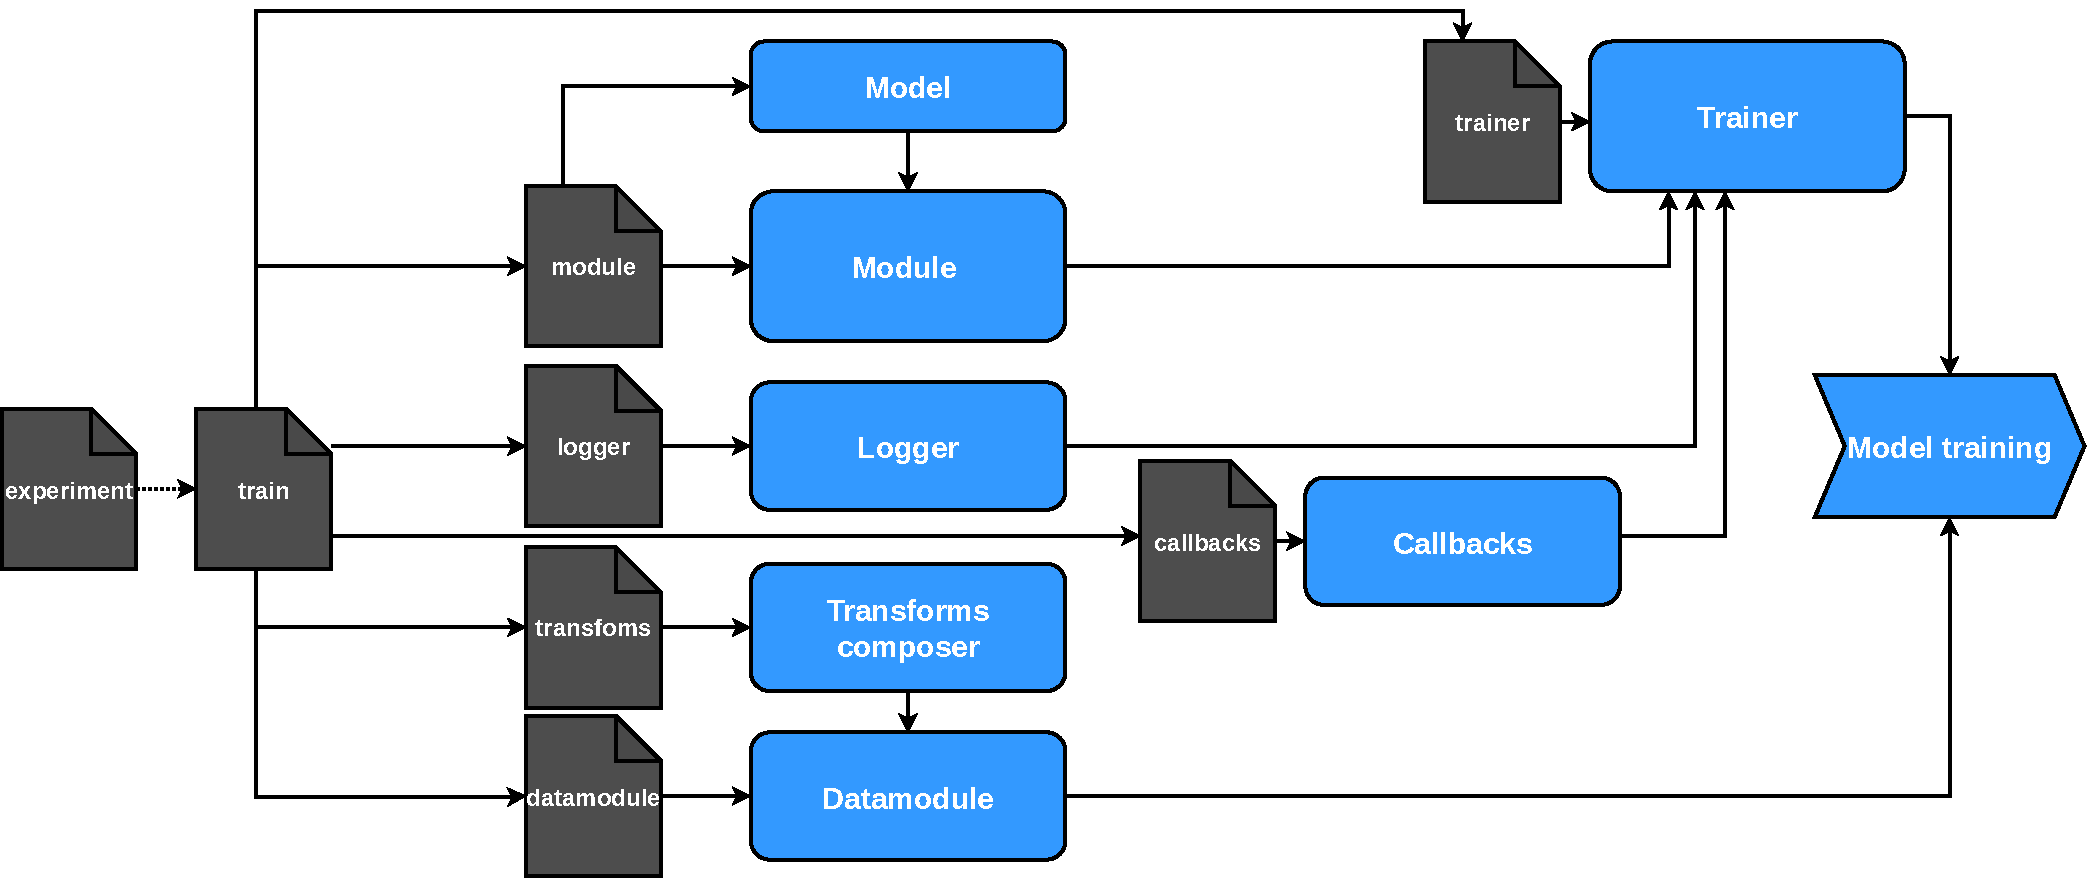
\includegraphics[width=\linewidth]{images/Module.drawio.pdf}
    \caption{Structure of modules and their configuration files}
    \label{fig:structure_modules}
\end{figure}

\begin{figure}
    \begin{forest}
        for tree={
        font=\ttfamily,
        grow'=0,
        child anchor=west,
        parent anchor=south,
        anchor=west,
        calign=first,
        inner xsep=7pt,
        edge path={
                \noexpand\path [draw, \forestoption{edge}]
                (!u.south west) +(7.5pt,0) |- (.child anchor) pic {folder} \forestoption{edge label};
            },
        before typesetting nodes={
                if n=1
                    {insert before={[,phantom]}}
                    {}
            },
        fit=band,
        before computing xy={l=15pt},
        }
        [MT
            [configs - root folder with all configuration files
                    [callbacks]
                    [datamodule]
                    [experiment]
                    [logger]
                    [module]
                    [trainer]
                    [transforms]
                    [train.yaml]
            ]
            [src - folder with all source files
                    [core - structures for data manipulation]
                    [data - utility functions for dataloaders and datasets]
                    [datamodules]
                    [models]
                    [modules]
                    [notebooks - \text{jupyter notebooks for auxilary tasks}]
                    [transforms - \text{classes to compose transformations given by configuration file}]
                    [utils  - \text{functions for logging, losses, data conversion}]
            ]
            [tests - contains multiple subfolders with unit tests for the program]
        ]
    \end{forest}
    \caption{Folder structure of the project}
    \label{fig:folder_structure}
\end{figure}
The object detection framework developed for this project was programmed in Python 3.8.12 \cite{Python}. We structured it into multiple independent modules, which can be swapped for their  corresponding alternatives. This ensures maximal reuse of the written code and allows further extension of this framework. This modular approach was inspired by MetaAI research \cite{MetaAIStatement} and IceVision library \cite{Icevision2022}. The framework's modularity will enable us to use it for semantic segmentation or classification problems.
The core of the project is the deep-learning framework PyTorch 1.11.0 \cite{Pytorch}, which is used to create and train neural networks. Although there are many open-source libraries with object detection frameworks, relying only on those libraries is far from optimal because the options to change the program's behavior are limited.
We, therefore, decided to write our framework. It handles all tasks required for training a model: Loading the data, model definition, optimization of the model, tracking the progress of training, etc.  Implementing all models from scratch would be ineffective; therefore, we support third-party models' usage. However, only the bare model is used. Thus, we can change everything except for the architecture of the model and its forward pass.

The project is divided into three folders: configurations, tests, and source (src). The first-mentioned contains YAML files that are further dispersed into dedicated folders based on the module they configure. At the root of the configuration folder are train.yaml and test.yaml files, which define how to compose individual modules to perform the target tasks. Hydra \cite{Yadan2019Hydra} handles the composition of configuration files. The user can override the default configuration from the command line or experiment.yaml file. The whole configuration pipeline can be seen in Figure \ref{fig:structure_modules}, and the project's folder structure is in Figure \ref{fig:folder_structure}.



\subsection{Models}
Models are implementations of one of the architectures described in section \ref{sec:deteciton_models}. We can either fully implement them, or we can rely on open-source libraries. In that case, we need to implement a function that transforms the data into the format required by the third-party model.

\subsection{Modules}
Modules are a wrapper around the model and they are based on Pytroch-Lightning modules \cite{falcon2019pytorch}. In modules, we take care of the following:
\begin{itemize}
    \item Training and validation loop
    \item Initialization of optimizer
    \item Initialization of learning rate schedulers
    \item Computing metrics
    \item Logging metrics to a predefined logger
    \item Transformations of outputs of models into the unified format
\end{itemize}


\subsection{Transformations}
Transformations are defined by their YAML configuration file. This file is passed to the transformation composer class, which creates training and validation transformations, which are then passed to a data module. We relied on the Albumentations library for individual image augmentations.

\subsection{Data-Modules}
Data modules are based on PyTorch-Lightning data modules. They consist of:
\begin{itemize}
    \item Dataset, where we load the data from the hard drive into the memory and parse the file with saved annotations. After loading the data, predefined transformations are applied.
    \item Functions that transform the loaded data into the format required by the model we are about to train.
    \item Definitions of data loaders, which are responsible for merging the data into chunks, so-called batches.
\end{itemize}
\subsection{Trainer}
Trainer defines properties of the training, such as the number of GPUS used for the training or a maximal number of epochs that training is allowed to undergo before terminating.

\subsection{Callbacks}
Callbacks add capabilities to the training pipeline without changing any code. Typical ones that we used were: Definition of stopping criteria, adjusting policy for saving weights of the model, or saving images with their predictions during the training.

\subsection{Logging}
A logger is software capable of storing and visualizing logged values. In the beginning, we used Tensorboard TODO, but soon we switched to Weights and Biases \cite{wandb}, and used them throughout the rest of the thesis.

\section{Additional open-source software}
Throughout the project, we used the libraries mentioned above as well as the following:
\begin{itemize}
    \item We used OpenCV \cite{opencv_library} computer vision library during the segmentation of dental restorations for operations such as: Adaptive thresholding, morphological operations, etc.
    \item Computer vision library Kornia \cite{eriba2019kornia} was used to perform morphological operations on PyTorch tensors quickly.
    \item MMDetection \cite{mmdetection} provides an implementation of multiple object detection models. We used their implementation of swin transformers, RetinaNet and Faster-RCNN
    \item During the computation of metrics, we used PyCOCOtools, an official \cite{pycocotools} implementation of MS COCO metrics. It had to be significantly modified to provide us with the required capabilities.
    \item To visualize predictions, we used Voxel Fiftyone \cite{moorefiftyone}. The program can be on a self-hosted server. We used this to share predictions of the model with MDDr. Tichý, who was thus able to assess those and decide if the dataset contains any erroneous annotations.
    \item For model ensembling, we used the methods implemented by the author of Weighted box fusion \cite{Solovyev2019}, and we further enhanced the capabilities of their methods.
    \item We used YOLOv5 models from the Ultralytics repository. \cite{glennjocher2020}.
\end{itemize}